\chapter{Live cell imaging of DNA damage responses correlated with chromatin compaction}
The advantage of FAI is in the fact that it could be useful for observing chromatin dynamics in live cells. Since we have introduced a 405nm laser in our widefield setup with the dual lamp housing (Fig. {\ref{fig:setup}}), we could microirradiate hoechst-sensitized HeLa H2B-EGFP cells, and cause a localized damage, and monitor the change in the global state of chromatin compaction. Using DNA damage markers, we can follow damage repair dynamics along with chromatin compaction states.

\begin{figure}[H]
    {\hfill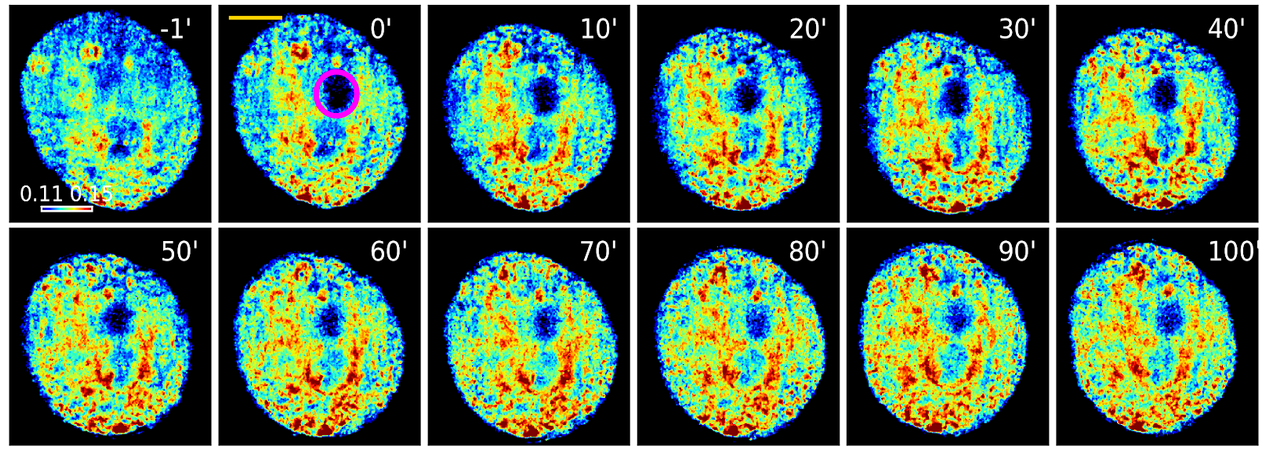
\includegraphics[clip,width=1\linewidth]{figures/live_an.png}\hspace*{\fill}}
    \caption{H2B-EGFP anisotropy of HeLa cells post microirradiation. Cells are microirradiated with 405nm laser (marked with purple circle), and imaged every 5 minutes for 2 hours. Scale bar corresponds to 5$\mu$m. Color bar is scaled for anisotropy values of 0.11 to 0.15}
    {\label{fig:live_an}}
\end{figure}
\section{Chromatin dynamics upon DDR}
\subsection{Chromatin compaction changes upon damage}
\subsection{Localization of histone and DDR proteins}
\section{Dynamics of repair and chromatin compaction}
\subsection{Chrombodies to visualize proteins}
\subsection{PARP and PCNA dynamics upon DDR}
\subsection{Repair and chromatin}
\paragraph*{} We microirradiated live cells and imaged them over 2 hours, every 5 minutes and computed their anisotropy maps (Fig. \ref{fig:live_an}). Since the 405nm laser bleaches EGFP locally, we could not obtain anisotropy information from the site of damage, but the anisotropy map of rest of the chromatin was unaffected. We quantified the change in anisotropy over time with $\Delta$Anisotropy, and found that as opposed to control (\(N=13\)), $\Delta$Anisotropy for irradiated cells (\(N=27\)) increased over time (Fig. \ref{fig:timetrace}). This indicated that there is increased compaction in the undamaged regions of chromatin in response to a local microirradiation. We fixed the cells after the course of imaging, and stained for common markers of DNA damage responses, and found that the phosphorylated form of DNA master kinase, ATM, forms nodes throughput the nucleus in a fraction of damaged cells (Fig. \ref{fig:patm}). These nodes are found in low anisotropy regions, indicating that these might be sites of damage repair. However, we were limited in observing the dynamics of repair factors, since fixing the cells destroys biological dynamics. In order to overcome this limitation, we utilized the chromobody technology (ChromoTek), and independently co-transfected H2B-EGFP expressing cells with chromobodies tagged with TagRFP against early and later markers of DDR, namely PARP1 and PCNA. Using this, we aimed to observe the dynamics of damage response in live cells, combined with chromatin compaction states as revealed by live anisotropy imaging.

\begin{figure}[H]
    {\hfill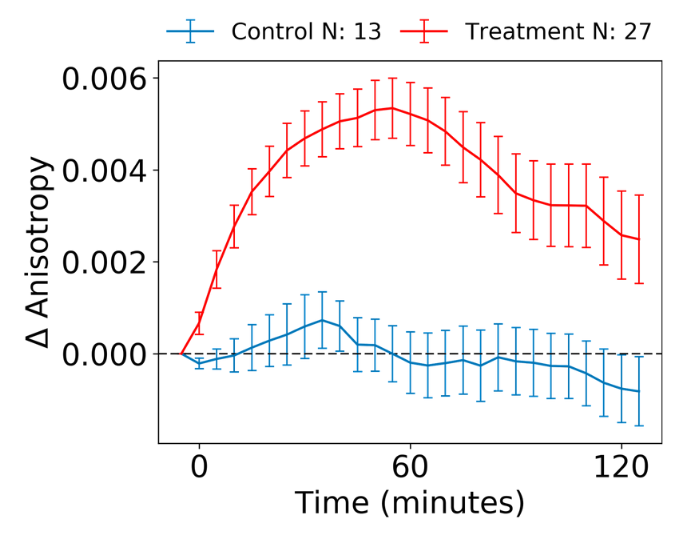
\includegraphics[clip, width=0.5\linewidth]{figures/timetrace.png}\hspace*{\fill}}
    \caption{$\Delta$Anisotropy is calculated by subtracting the mean anisotropy of any time point, with the mean anisotropy of the first time point for that cell. A positive $\Delta$Anisotropy corresponds to compaction, whereas a negative $\Delta$Anisotropy corresponds to decompaction.}
    {\label{fig:timetrace}}
\end{figure}

\begin{figure}[H]
    {\hfill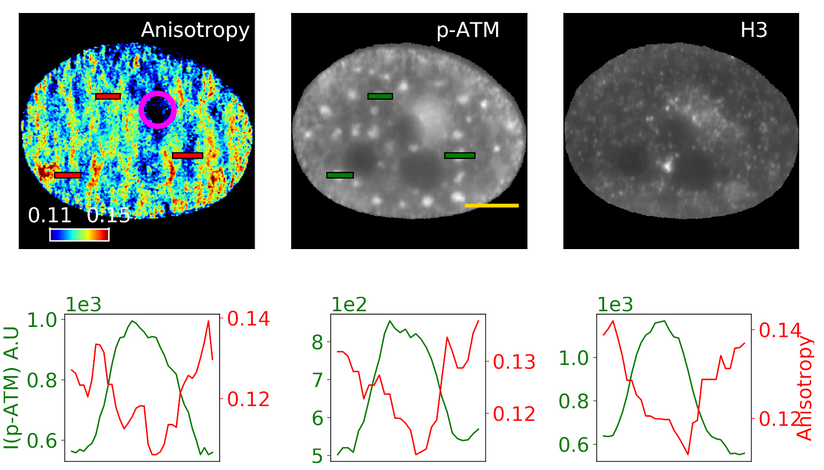
\includegraphics[clip, width=1\linewidth]{figures/patm.png}\hspace*{\fill}}
    \caption{Microirradiated cells are fixed after live imaging, and stained for damage markers. Phosphorylated-ATM is seen at sites of low anisotropy regions, and Histone H3 is accumulated at the site of damage. The purple circle is the site of microirradiation.}
    {\label{fig:patm}}
\end{figure}

\paragraph*{} PARP1 is a well characterized member of the poly (ADP ribose) polymerase (PARP) family of proteins, which are known to be transiently enhanced at sites of damage post microirradiation \cite{chou2010chromatin, qi2019multiple}. PARP1 is activated in the presence of broken DNA, which leads to the formation of poly (ADP ribose) (PAR), upon which further downstream repair factors are recruited. PCNA (proliferating cell nuclear antigen), a ring-shaped DNA replication cofactor, is a member of the family of DNA sliding clamps. It encircles DNA during replication, and enhances the processivity of DNA polymerase. PCNA is known to be associated with the final stages of DDR when new DNA has to be synthesized post excision of damaged DNA \cite{moldovan2007pcna}.

\begin{figure}[H]
    {\hfill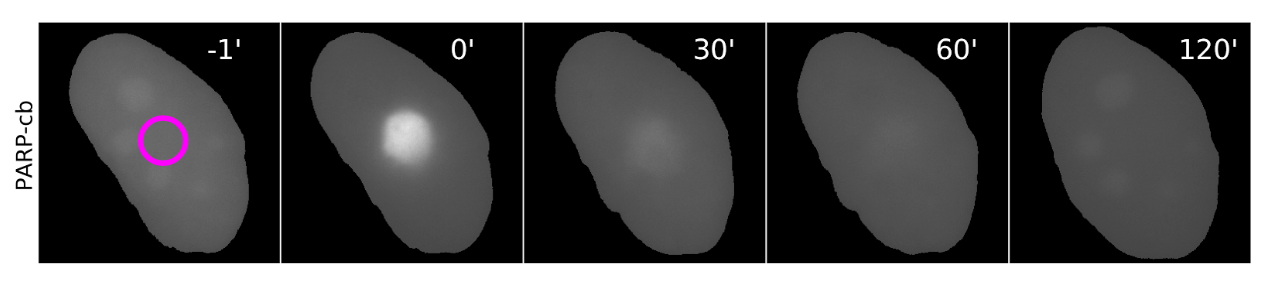
\includegraphics[clip, width=1\linewidth]{figures/parp.png}\hspace*{\fill}}
    \caption{Live cell dynamics of PARP-chrombody in irradiated cells, transiently transfected in HeLa H2B-EGFP cells. PARP1 showed immediate transient encrichment at the site of damage, and became homogenous quickly.}
    {\label{fig:parp}}
\end{figure}

\begin{figure}[H]
    {\hfill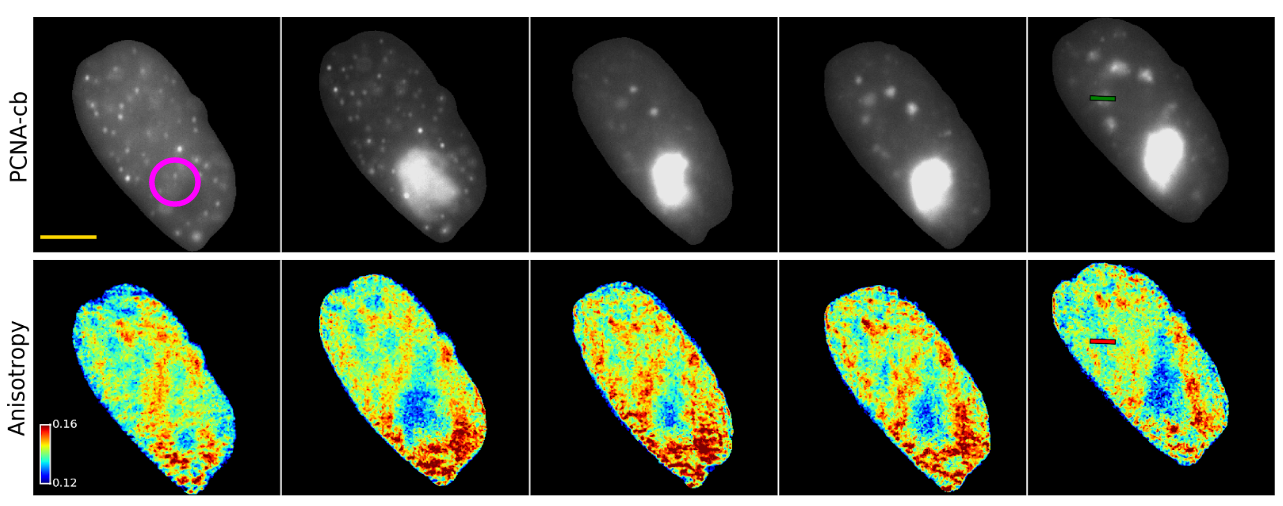
\includegraphics[clip, width=1\linewidth]{figures/pcna.png}\hspace*{\fill}}
    \caption{HeLa H2B-EGFP cells expressing PCNA chromobody along with its corresponding anisotropy maps, imaged at an  interval of 5 minutes post-irradiation. Scale bar corresponds to 5$\mu$m. Timestamps are same as (Fig. \ref{fig:parp})}
    {\label{fig:pcna}}
\end{figure}


\paragraph*{} We found that PARP1 was almost immediately recruited to site of damage upon microirradiation (Fig. \ref{fig:parp}), and diffused away from the site 15 minutes after damage. However, PCNA, which is a late stage repair protein, was also recruited immediately to the site of damage, and was found to be persistent at site of damage(Fig. \ref{fig:pcna}). We captured this behavior by quantifying the mean intensity of the chromobody at the site of damage, normalized to the mean intensity outside. (Fig. \ref{fig:retention})

\paragraph*{} While PCNA persists longer at the site of damage, within 20 minutes of irradiation, there are nodes of PCNA formed away form the site of damage. These nodes correspond to low-anisotropy regions, and incorporate EdU (ethynyl deoxyuridine), a thymidine analogue for labelling proliferating cells, suggesting that they are sites of damage repair.

\begin{figure}[H]
    {\hfill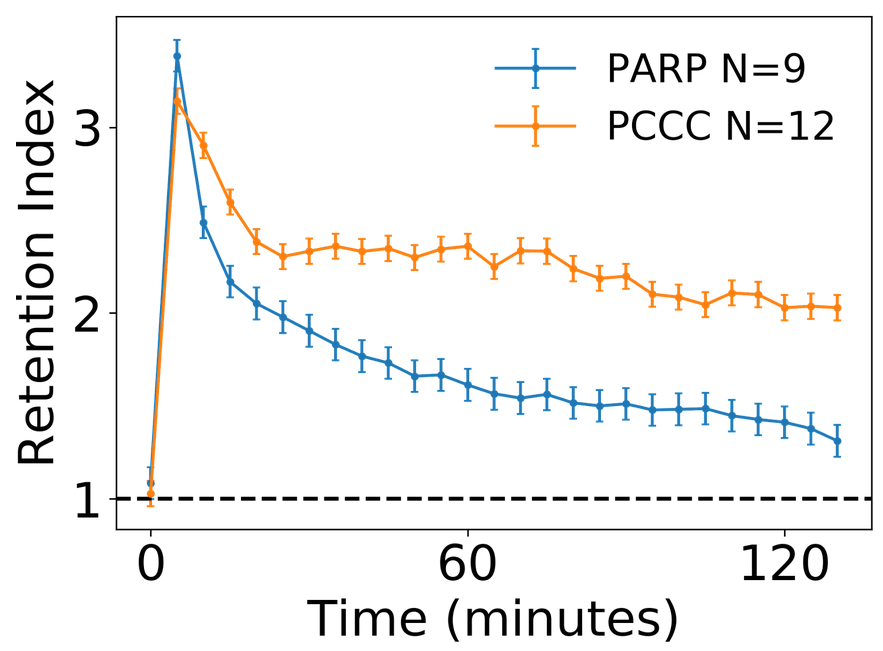
\includegraphics[clip, width=0.5\linewidth]{figures/retention.png}\hspace*{\fill}}
    \caption{PCNA persists at the site of damage longer than PARP. Retention index of any time point is defined as the ratio of intensity for a chromobody at the site of damage and outside the site of damage.}
    {\label{fig:retention}}
\end{figure}

\paragraph*{} We noticed that within 2 min after microirradiation, there is phosphorylation of Ser139 of the histone variant H2AX at the site of microirradiation, indicating DNA damage (Supplemental Figure 4). Although $\Gamma$H2AX is a DNA damage marker, which is generally found as foci in regions of damaged chromatin, there is also a pan-nuclear spreading of $\Gamma$H2AX in undamaged chromatin as early as 5 min after damage. In another study, interference with chromatin compaction at the damage site reduces the efficiency of damage repair. This suggested that condensation of chromatin is a necessary step in the activation of DDR (Burgess et al., 2014). However, ATM activation in mouse fibroblasts showed chromatin opening independent of DNA damage (Ji et al., 2017). During damage, ATM is thought to be activated not by direct binding to DNA strand breaks, but by changes in chromatin structure. Thus, forced compaction of chromatin promotes activation of ATR and ATM even where there are no strand breaks (Burgess et al., 2014), and conversely, activation of these kinases can change chromatin compaction (Becker et al., 2014). Thus, pan-nuclear induction of DDR (for which $\Gamma$H2AX is a proxy) can drive compaction of undamaged chromatin, and the processes could feed back onto each other.

Such pan-nuclear induction of $\Gamma$H2AX has been reported before when clustered DNA damage was induced by ionizing radiation, which is regulated by ATM and DNA-PK (Meyer et al., 2013). Other studies have discussed a ring of $\Gamma$H2AX in the context of apoptosis (Solier and Pommier, 2014). It is possible that some of the cells we have irradiated will undergo apoptosis, and apoptotic response over and above the DNA damage response complicates the observed chromatin phenotypes. But apoptosis is accompanied by visible changes in the cell and nuclear morphology. However, our irradiated cells, under similar irradiation conditions, do not exhibit apoptotic morphology or fragmented chromatin, and many survive 48 h after irradiation. Furthermore, during the 2-h time course over which the cells were imaged, there was no significant induction of apoptotic or general cell death markers (Supplemental Figure 9). This indicates that the compaction we observe may have to do with the early processes of DDR rather than the long-term processes of cell death because of excessive DNA damage.

PCNA, surprisingly, is shown to be recruited immediately to the site of localized DSBs, independent of cell-cycle phase. As interestingly, at longer time-points it forms transient nodes of repair away from the site of damage in regions of more open chromatin (low anisotropy). These nodes actively incorporate EdU, indicating active repair and possibly a looping of DSBs from the primary laser-induced cluster to open regions of chromatin for the purposes of repair.

Our study establishes the possibility of using FAI to measure chromatin compaction changes in the context of DNA damage in living cells, followed by immunofluorescence for DDR and chromatin markers. While the response to DSBs is investigated here, following previous studies (Kruhlak et al., 2006; Burgess et al., 2014), in principle, the method is amenable to other forms of DNA damage as well, which we aim to investigate in the future.

\paragraph*{} In summary, we observed the dynamics of chromatin compaction state, and correlated it with markers of damage, such as phosphorylated ATM, which forms nodes at low anisotropy regions. We found that damage repair markers have different dynamics, as PARP1 has low retention in the site of damage, as opposed to PCNA, which persists for longer time period. We also observed that PCNA forms nodes of repair, away from the site of damage, which correspond to regions of low anisotropy and EdU incorporation.

